\documentclass[tikz,border=2pt]{standalone}
\usepackage{amsmath}
\usepackage{pgfplots}
\pgfplotsset{compat=1.18}
\usetikzlibrary{arrows.meta}

\begin{document}
% Taylor's theorem for f(x)=e^x at a=0 with k=2: f(x) = T_2(x) + R_2(x), where T_2 is the
% quadratic approximation and the remainder R_2(x) (the gap) is of order x^3.
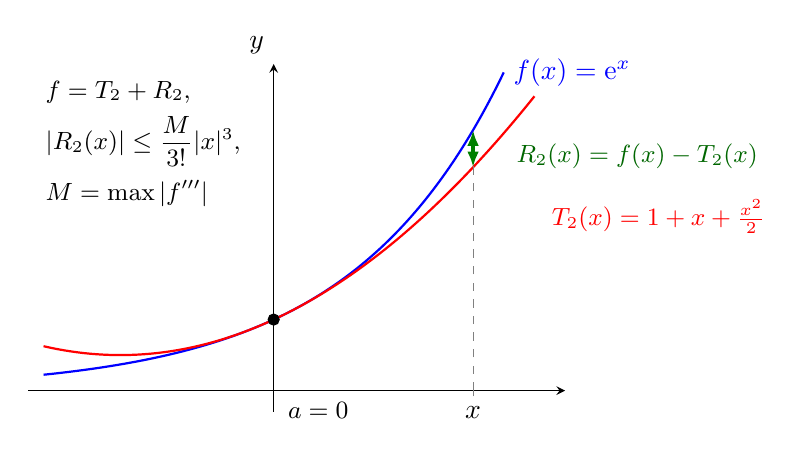
\begin{tikzpicture}
	\begin{axis}[
		axis lines=middle,
		xmin=-1.6, xmax=1.9,
		ymin=-0.3, ymax=4.6,
		xtick={1.3}, xticklabels={$x$}, ytick=\empty,
		xlabel={}, ylabel={$y$},
		ylabel style={above left},
		samples=120, smooth, clip=false,
		width=8.4cm, height=6cm
		]
		\addplot[thick, blue, domain=-1.5:1.5] {exp(x)};
		\addplot[thick, red, domain=-1.5:1.7] {1+x+x^2/2};
		\addplot[only marks, mark=*, black] coordinates {(0,1)};
		\draw[dashed, gray] (axis cs:1.3,0) -- (axis cs:1.3,3.669);
		\draw[{Latex[length=2mm]}-{Latex[length=2mm]}, green!50!black, very thick] (axis cs:1.3,3.145) -- (axis cs:1.3,3.669);
		\node[green!40!black, anchor=west, font=\small] at (axis cs:1.52,3.3) {$R_2(x)=f(x)-T_2(x)$};
		\node[blue, anchor=west] at (axis cs:1.5,4.48) {$f(x)=\mathrm{e}^x$};
		\node[red, anchor=west, font=\small] at (axis cs:1.75,2.45) {$T_2(x)=1+x+\tfrac{x^2}{2}$};
		\node[anchor=north west, font=\small, align=left] at (axis cs:-1.55,4.5) {$f=T_2+R_2$,\\[4pt] $|R_2(x)|\le\dfrac{M}{3!}|x|^3$,\\[4pt] $M=\max|f'''|$};
		\node[anchor=north west, font=\small] at (axis cs:0.03,-0.03) {$a=0$};
	\end{axis}
\end{tikzpicture}
\end{document}
